
\subsection{SWAP accounting with chequebook}

Nonetheless, even in this simple form, the chequebook proves quite useful.
\cite{ethersphere2016sw3} introduces a protocol for peer-to-peer accounting, called \gloss{swap}.
\gloss{swap} is a tit-for-tat accounting scheme that scales microtransactions by
allowing service for service exchange between connected peers
(\emph{swap = swarm accounting protocol for service wanted and provided}).

In case of equal consumption with low variance over time, bidirectional services can be accounted for without any payments. Data relaying is an example of such a service, making swap
ideally suited for implementing bandwidth incentives in content delivery or mesh networks.

\begin{center}
\begin{figure}
\begin{center}
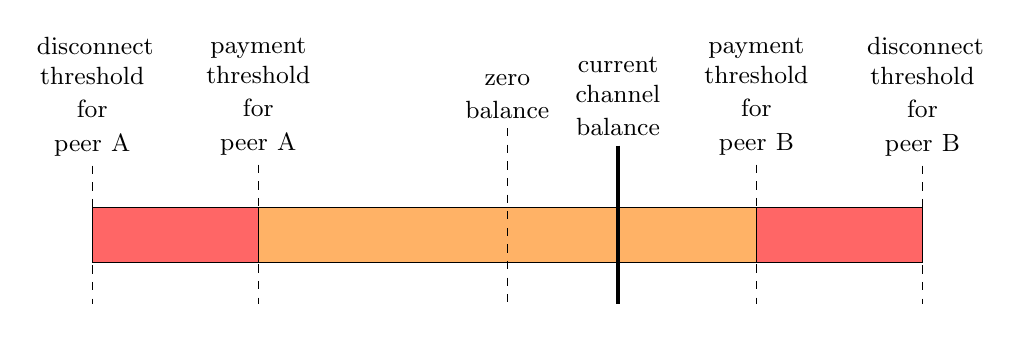
\begin{tikzpicture}
\node (middle)[draw, rectangle, fill=orange!60, minimum height=2em, minimum width=18em]{};
\node (leftred) [draw, rectangle, fill=red!60, minimum height=2em, minimum width=6em, node distance=12em,left of=middle]{};
\node (rightred)[draw, rectangle, fill=red!60, minimum height=2em, minimum width=6em, node distance=12em,right of=middle]{};
\node (zero) [above of=middle,node distance=5em, text width=4em, align=center] {\small zero\\ balance};
\node (zerod) [below of=middle] {};
\draw [dashed](zero)--(zerod);
\node (rtol) [node distance=9em,right of=zero,text width=4em, align=center] {\small payment\\threshold\\for peer B};
\node (rtold) [node distance=9em,right of=zerod] {};
\node (ltol) [node distance=9em,left of=zero,text width=4em, align=center] {\small payment\\threshold\\for peer A};
\node (ltold) [node distance=9em,left of=zerod] {};
\node (rdis) [node distance=15em, right of=zero,text width=4em, align=center] {\small disconnect\\threshold\\for peer B};
\node (rdisd) [node distance=15em,right of=zerod] {};
\node (ldis) [node distance=15em, left of=zero,text width=4em, align=center] {\small disconnect\\threshold\\for peer A};
\node (ldisd) [node distance=15em,left of=zerod] {};
\node (rbal) [node distance=4em,right of=zero,text width=4em, align=center] {\small current\\channel\\balance};
\node (rbald) [node distance=4em,right of=zerod] {};

\draw [dashed](rtol)--(rtold);
\draw [dashed](ltol)--(ltold);
\draw [dashed](rdis)--(rdisd);
\draw [dashed](ldis)--(ldisd);
\draw [very thick](rbal)--(rbald);
\end{tikzpicture}
\end{center}
\caption{Swap balance and swap thresholds.
Zero balance in the middle indicates consumption and provision are equal.
The current channel balance represents the difference in uncompensated service provision:
if to the right of zero, the balance tilts in favour of A with peer B being in debt, whereas to the left
the balance tilts in favour of B with A being in debt.
The orange interval represents loss tolerance. If the balance goes over the payment threshold, the party in
debt sends a cheque to its peer, if it reaches the disconnect threshold, the peer in debt is disconnected.}
\label{fig:swap}
\end{figure}
\end{center}


Extended with a delayed payment instrument like the chequebook, swap also offers a way to deal with unequal consumption as well as high variance.
In the presence of high variance, or unequal consumption of services, the balance will eventually tilt significantly toward one peer. In this situation, the indebted
party issues a cheque to the creditor to return the nominal balance to zero. This process is automatic and justifies swap as \emph{settle (the balance) with automated payments}
(see figure \ref{fig:swap}).

Such cheques can be cashed immediately by being sent to the issuer's chequebook contract. Alternatively, cheques can also be withheld
%. Withholding a cheque is effectively lending on credit, 
which enables the parties to save on transaction costs.
While, strictly speaking, there are no solvency guarantees, a bounced cheque will affect the issuer's reputation as the chequebook contract records it.
On the premise that cheques are swapped in the context of repeating dealings, peers will refrain from issuing cheques beyond their balance. In other words, interest in keeping good reputation with their peers serves as an incentive for nodes to maintain solvency.

\begin{center}
\begin{figure}
\begin{center}
\begin{tabular}{ccc}
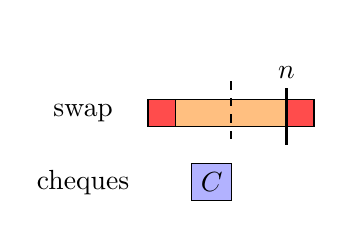
\begin{tikzpicture}
\node (middle)[draw, rectangle, fill=orange!50, minimum height=1em, minimum width=4em]{};
\node (leftred) [draw, rectangle, fill=red!70, minimum height=1em, minimum width=1em, node distance=2.5em, left of=middle]{};
\node (rightred)[draw, rectangle, fill=red!70, minimum height=1em, minimum width=1em, node distance=2.5em, right of=middle]{};
\node (zero) [above of=middle,node distance=2em, text height=1em] {};
\node (zerod) [below of=zero, node distance=3.5em] {};
\node (balance) [right of=zero,node distance=2em, text height=1.5em] {$n$};
\node (balanced) [below of=balance,node distance=3.5em] {};
\draw [dashed](zero)--(zerod);
\draw [very thick](balance)--(balanced);
\node (payment) [below of=zerod, node distance=1em]{};
\node (cheqeue) [draw, left of=payment, node distance=.7em, minimum height=1em, minimum width=1.4em, fill=blue!30, rectangle]{$C$};

\node (swap) [left of=leftred,minimum width=1em,align=right]{swap};
\node (cheques) [below of=swap,minimum width=1em, node distance= 2.5em, align=right]{cheques};
\end{tikzpicture}
&
\begin{tabular}{c}
  $\Longrightarrow$
\\ \\ \\ \\
\end{tabular}
&
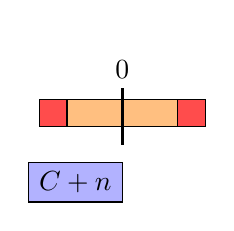
\begin{tikzpicture}
\node (middle)[draw, rectangle, fill=orange!50, minimum height=1em, minimum width=4em]{};
\node (leftred) [draw, rectangle, fill=red!70, minimum height=1em, minimum width=1em, node distance=2.5em, left of=middle]{};
\node (rightred)[draw, rectangle, fill=red!70, minimum height=1em, minimum width=1em, node distance=2.5em, right of=middle]{};
\node (zero) [above of=middle,node distance=2em, text height=1.5em] {$0$};
\node (zerod) [below of=zero, node distance=3.5em] {};
% \draw [dashed](zero)--(zerod);
\draw [very thick](zero)--(zerod);
\node (payment) [below of=zerod, node distance=1em]{};
\node (cheque) [draw, left of=payment, node distance=1.7em, minimum height=1em, minimum width=3.4em, fill=blue!30, rectangle]{$C+n$};
\end{tikzpicture}
\end{tabular}
\end{center}

\caption{Peer B's swap balance (with respect to A) reaches the payment threshold $n$ (left),
B sends a cheque to peer A. B keeps the cheque and restores the swap balance to zero.}
\label{fig:chequeswap}
\end{figure}
\end{center}